\subsubsection{Attori primari}
	\begin{figure}[h!]
		\centering
		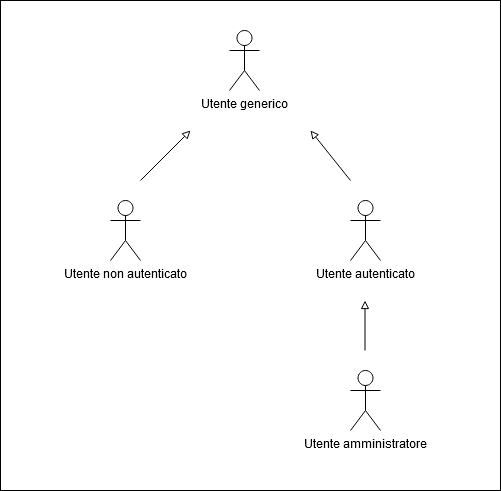
\includegraphics[width=10cm]{images/diagramma_attori.png}
		\caption{Diagramma degli attori}
	\end{figure}

	Gli attori primari sono classificati nella maniera seguente:
	\begin{itemize}
		\item \textbf{Utente generico}: utente che interagisce con il sistema;
		\item \textbf{Utente non autenticato}: utente che interagisce con il sistema e che non risulta essere autenticato. Implica la possibilità che un utente sia registrato nel sistema ma non abbia ancora effettuato la procedura di login;
		\item \textbf{Utente autenticato}: utente che interagisce con il sistema e che risulta essere autenticato dopo aver svolto la procedura di login;
		\item \textbf{Utente amministratore}: utente che interagisce con il sistema, che risulta essere autenticato dopo aver svolto la procedura di login e che possiede i privilegi per accedere a sezioni dedicate del sistema (in particolare, quelle dedicate alla modifica).
	\end{itemize}